\subsection{Software Attestation Overview}

The security of systems that employ trusted processors hinges on
\textit{software attestation}. The software running inside an \textit{isolated
container} established by trusted hardware can ask the hardware to sign a
small piece of \textit{attestation data}, producing an
\textit{attestation signature}. Asides from the attestation data, the signature
includes a \textit{measurement} that uniquely identifies the software inside
the container. Therefore, an attestation signature can be used to convince a
\textit{verifier} that the attestation data was produced by a specific piece
of software, which is hosted inside a container that is isolated from outside
interference by trusted hardware.

Each hardware platforms discussed in this section uses a slightly different
software attestation scheme. Platforms differ by the amount of software that
executes inside an isolated container, by the isolation guarantees provided to
the software inside a container, and by the process used to obtain a
container's measurement. The threat model and security properties of each
trusted hardware platform follow directly from the design choices outlined
above, so a good understanding of attestation is a prerequisite to discussing
the differences between existing platforms.

Software attestation can be used to authenticate one party in a key exchange
protocol. The resulting protocol can assure a verifier that it is communicating
over a secure channel with a specific piece of software, hosted inside an
isolated container created by trusted hardware. The next paragraph outlines the
augmented protocol, using Diffie-Hellman Key Exchange (DKE)
\cite{diffie1976keyexchange} as an example key exchange protocol.

The verifier starts executing the key exchange protocol, and sends the first
message, $g^{A}$, to the software inside the secure container. The software
inside the container produces the second key exchange message, $g^{B}$, and
asks the trusted hardware to attest the cryptographic hash of both key exchange
messages, $h(g^{A} || g^{B})$. The verifier receives the second key exchange
and attestation signature, and authenticates the software inside the secure
container by checking all the signatures along the \textit{attestation chain}
of trust shown in Figure~\ref{fig:generic_attestation_chain}.

\begin{figure}[hbt]
  \centering
  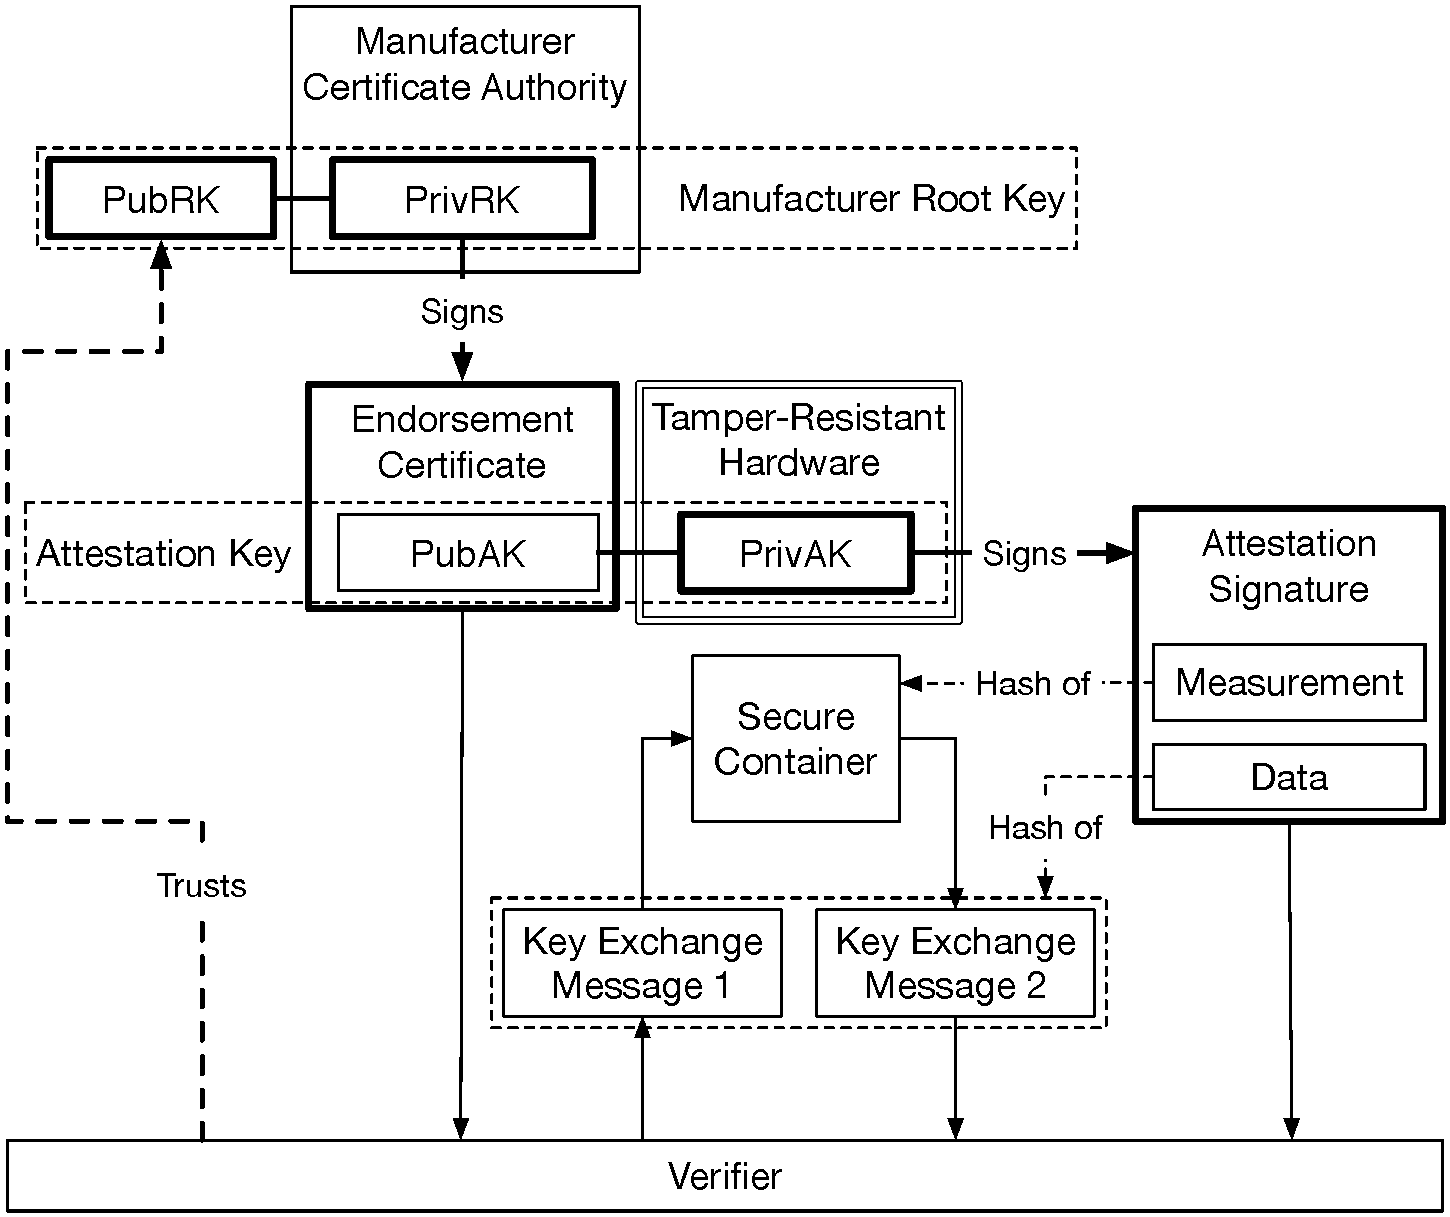
\includegraphics[width=85mm]{figures/generic_attestation_chain.pdf}
  \caption{
    The chain of trust in software attestation. The root of trust is a
    manufacturer key, which produces an endorsement certificate for the secure
    processor's attestation key. The processor uses the attestation key to
    produce the attestation signature, which contains a cryptographic hash of
    the container and a message produced by the software inside the container.
  }
  \label{fig:generic_attestation_chain}
\end{figure}

The chain of trust used in software attestation is rooted at a signing key
owned by the hardware manufacturer, which must be trusted by the verifier. The
manufacturer acts as a Certificate Authority (CA), and provisions each secure
processor that it produces with a unique \textit{attestation key}, which is
used to produce \textit{attestation signatures}. The manufacturer also
generates an \textit{endorsement certificate} for each secure processor,
by signing the public part of the processor's attestation key with the
manufacturer \textit{root key}. When the verifier receives a valid endorsement
certificate signed by a manufacturer key that it trusts, the verifier is
assured that the private part of the attestation key in the certificate is
stored in tamper-resistant hardware, and is only used for producing attestation
signatures, under the rules set by the trusted manufacturer.

A secure processor identifies each isolated container by storing a
cryptographic hash of the code executed inside the container. When the
processor is asked to sign a piece of attestation data, it uses the
cryptographic hash associated with the container as the measurement in the
attestation signature. After a verifier validates the processor's attestation
key using its endorsement certificate, the verifier ensures that the signature
is valid, and that the measurement in the signature belongs to the software
that it expects to communicate with. Having checked all the links in the
attestation chain, the verifier has authenticated the other party in the key
exchange, and is assured that it now shares a secret with the software that it
expects, running in an isolated container on hardware that it trusts.
